\section{Methodology}\label{sec:method}
\subsection{Visibility and initial fragments}
The receiver checks a contiguous evidence-ledger sequence, one availability record per alert, consistency between alert and ledger availability, and absence of private fields. It retains alerts and claims available by $T=100$, including only claims whose two endpoints are eligible. The initial correlator forms same-source and process-tree groups and tests available lineage references. Its host/account and component-cap guards operate on the current components; the standalone claim verifier does not retrospectively certify every initial within-source pair. Thus the zero false-pair observation is an evaluated property of this holdout, not a theorem of the verifier.

\subsection{Original independent attestation}
Claims are bundled by relationship token. The baseline's additional cross-fragment union requires exactly one original claim from each family $\{\mathrm{process},\mathrm{authentication},\mathrm{network}\}$, three distinct upstream roots, availability by $T$, identical endpoint/event identities, matching host/account, temporal compatibility, and matching process-parent, session, and flow identifiers. The event-time guard requires $t_b\geq t_a-3$ and $|t_b-t_a|\leq25$ minutes. A derived claim cannot replace an original family. Before union, the current components must share a host and an account and their combined size must not exceed 100.

The root and visibility checks are necessary conditions:
\begin{equation}\label{eq:gate}
\left|\{\rho(c):c\in B_r,\;c\text{ original}\}\right|=3,\qquad
\max_{c\in B_r}t_{\mathrm{available}}(c)\leq T.
\end{equation}
Equation~\ref{eq:gate} does not alone imply acceptance: all identity, context, time, and component checks must also pass. The verifier logs a failed reason and leaves the partition unchanged. Each token's attestation is checked against original alert fields; newly joined components do not create synthetic support for a subsequent token. Union operations themselves are transitive, so the final group can contain alerts joined through multiple separately checked tokens.

\subsection{Constrained endpoint fallback}
The candidate retries only rejected tokens with reason \texttt{missing\_family}. It requires exactly two original claims, one authentication and one network-flow claim, with distinct roots and availability by 100. The two endpoint alerts must themselves be original, from different source and observation identifiers, with a common endpoint-origin root that differs from both claim roots. Their host, account, event timing, process-parent, authentication-session, and flow identifiers must agree. Every claim in the bundle must agree with endpoint fields; component host/account overlap and cap checks are reapplied. The endpoint observation serves as the missing process-family witness. Other rejection reasons are not relaxed. Figure~\ref{fig:verify} traces these gates.
\begin{figure}[ht]\centering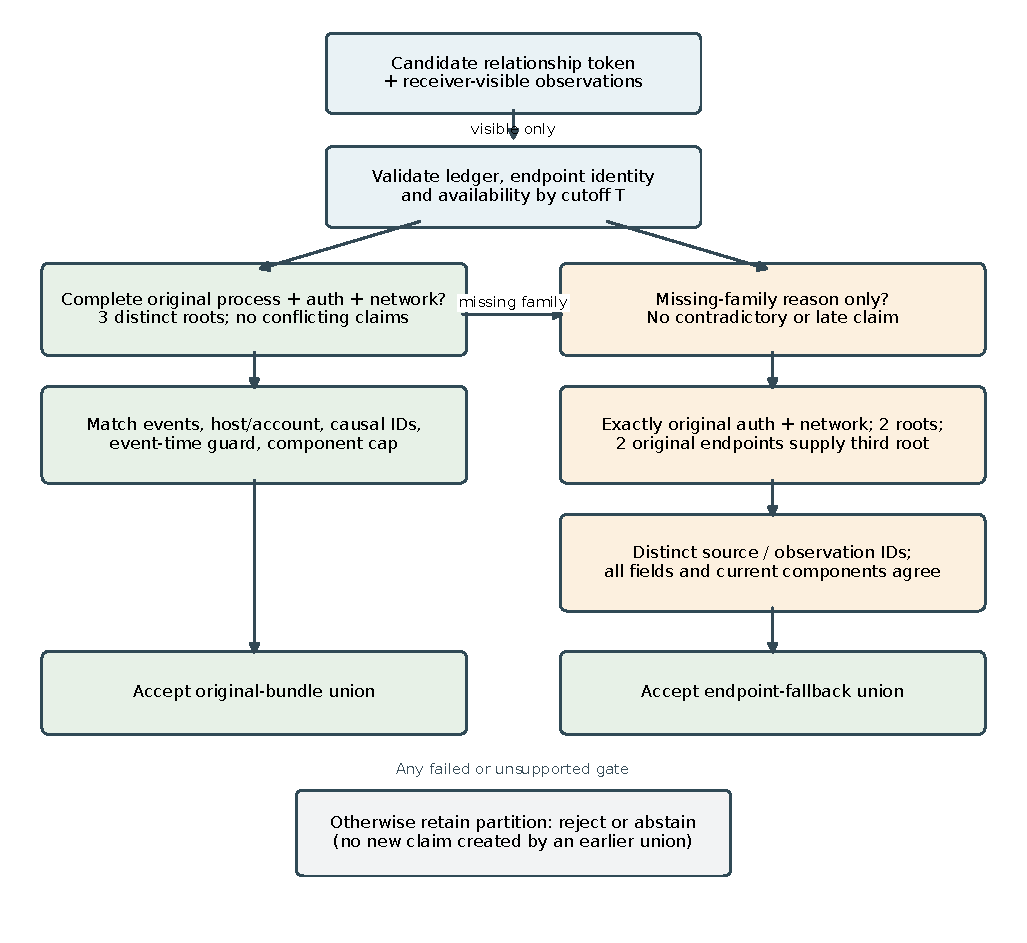
\includegraphics[width=\linewidth]{figures/verification_methodology.pdf}\caption{Relationship-token verification. A complete original process/authentication/network bundle can pass the baseline verifier. Only a missing-process-family rejection enters the endpoint fallback, which requires two original claim roots plus a third endpoint root. Identity, field, temporal, component-context, and size checks remain mandatory. Failed or unsupported tokens do not change the existing groups.}\label{fig:verify}\end{figure}

\subsection{Grouping and scoring}
Both arms rank by source depth: $1.2$ times maximum severity, $0.7$ times maximum asset criticality, $0.55$ times distinct event types, and $0.7$ times the number of distinct sources capped at 10. The frozen baseline adds one point per accepted token whose left endpoint is in the group. The candidate uses the same bonus coefficient of one and includes fallback unions. Groups are sorted by descending score and then first alert identifier. A group never becomes recoverable merely because its rank changes; Figure~\ref{fig:groups} separates grouping from top-20 retrieval.
\begin{figure}[ht]\centering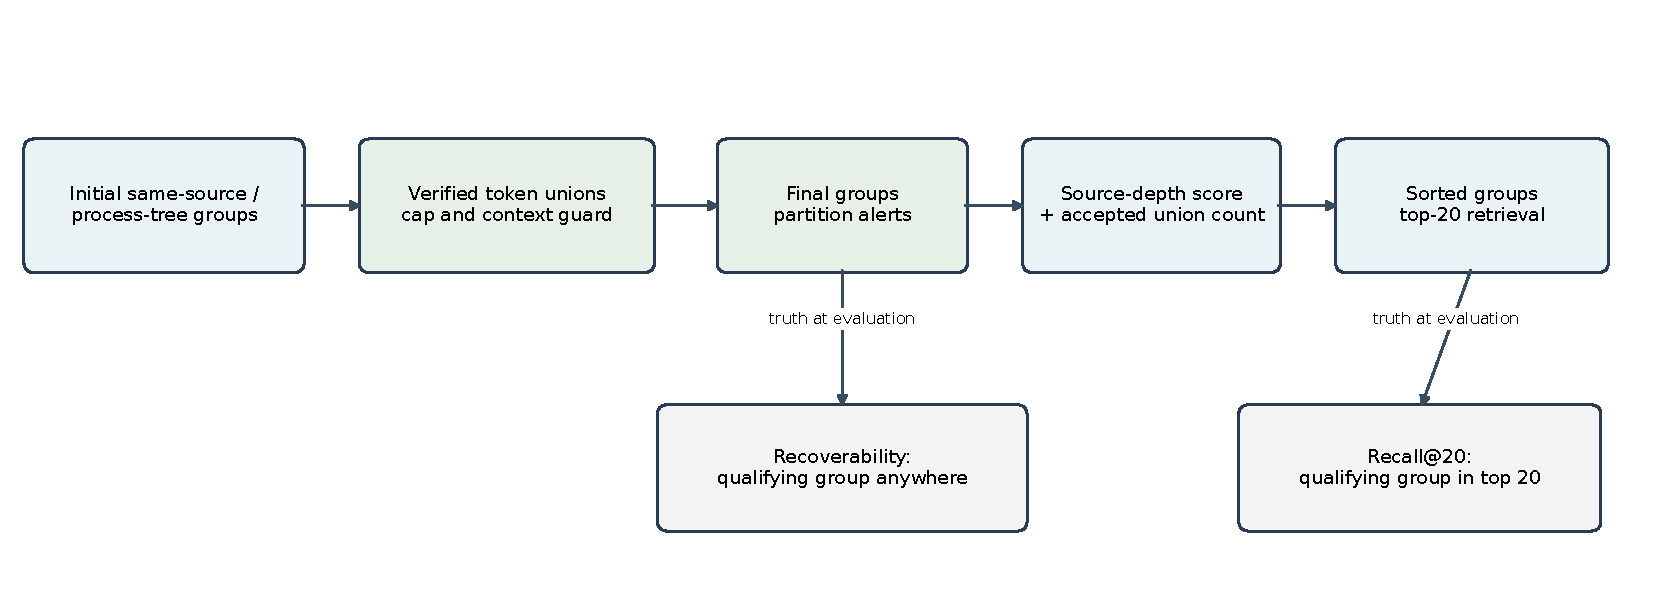
\includegraphics[width=\linewidth]{figures/reconstruction_prioritization.pdf}\caption{Initial fragments and accepted evidence-token unions form the final partition. Scoring orders these fixed groups. The evaluator separately checks whether an expert incident has a sufficiently complete and pure group anywhere (recoverability) and whether one appears within the first 20 (Recall@20); ranking cannot create a missing group.}\label{fig:groups}\end{figure}
